An easy way to glance at recurrent event data is by event plots, which
can be created by applying the generic function \texttt{plot()} to the
\texttt{Recur} object when the \pkg{reReg} package is loaded.
Additionally, the \texttt{plotEvents()} function from the \pkg{reReg}
package allows users to stratify the event plots by discrete variables.
The following codes produces event plots with and without stratifying by
if the patients received chemotherapy.

\begin{Shaded}
\begin{Highlighting}[]
\NormalTok{df0 <-}\StringTok{ }\KeywordTok{subset}\NormalTok{(readmission, !(id %in%}\StringTok{ }\KeywordTok{c}\NormalTok{(}\DecValTok{60}\NormalTok{, }\DecValTok{109}\NormalTok{, }\DecValTok{280}\NormalTok{)))}
\NormalTok{obj <-}\StringTok{ }\KeywordTok{with}\NormalTok{(df0, }\KeywordTok{Recur}\NormalTok{(t.stop, id, event, death))}
\KeywordTok{plot}\NormalTok{(obj, }\DataTypeTok{legend =} \StringTok{"top"}\NormalTok{) }\CommentTok{# Figure 1}
\NormalTok{fn <-}\StringTok{ }\KeywordTok{Recur}\NormalTok{(t.stop, id, event, death) ~}\StringTok{ }\NormalTok{chemo}
\KeywordTok{plotEvents}\NormalTok{(fn, }\DataTypeTok{data =} \NormalTok{df0, }\DataTypeTok{legend =} \StringTok{"top"}\NormalTok{) }\CommentTok{# Figure 2}
\end{Highlighting}
\end{Shaded}

\vspace*{-.3cm}\begin{figure}[H]
    \centering
    \begin{minipage}{0.24\textwidth}
        \centering
        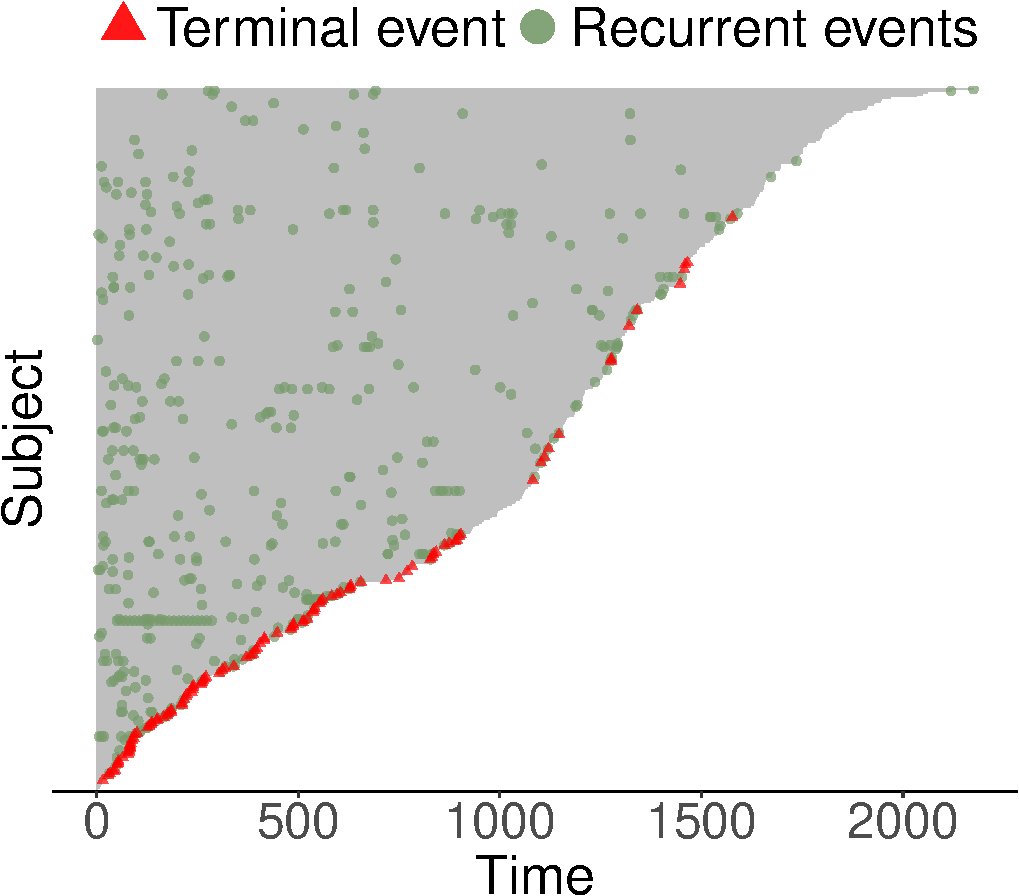
\includegraphics[scale = .25]{recur-figs/ep-1}
        \caption{No stratification}
    \end{minipage}\hfill
    \begin{minipage}{0.24\textwidth}
        \centering
        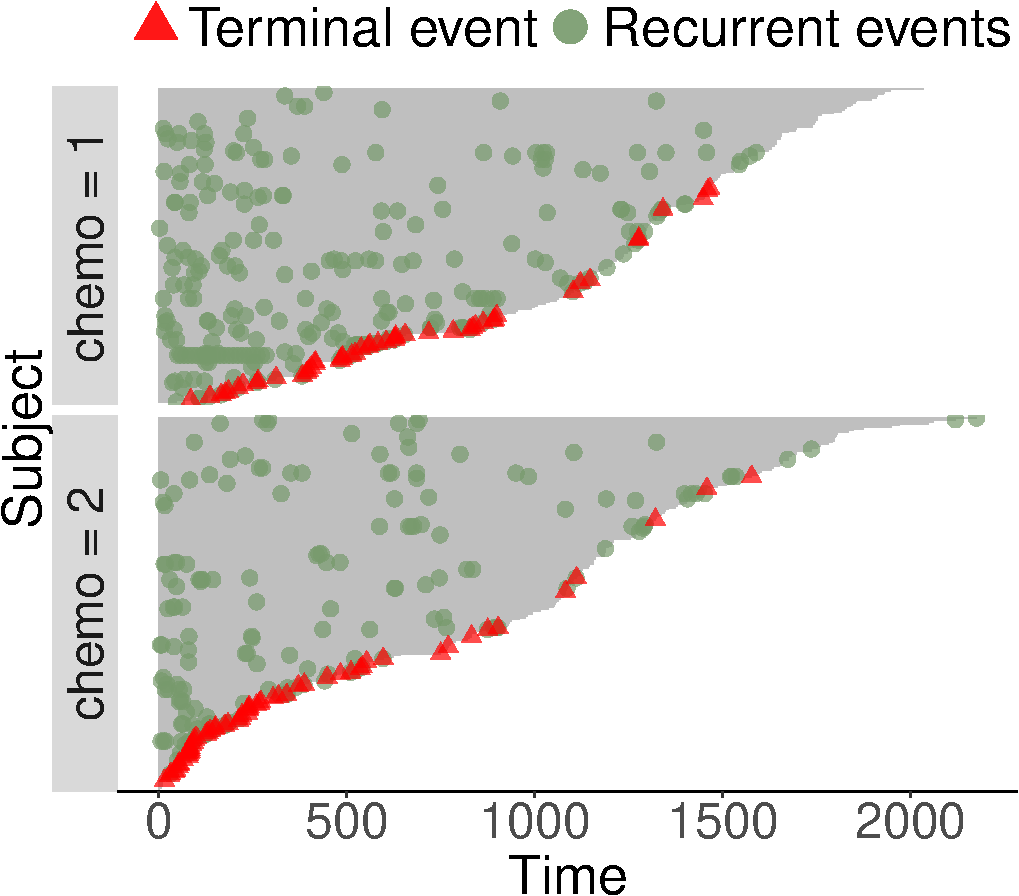
\includegraphics[scale = .25]{recur-figs/ep-2}
        \caption{Stratified by \texttt{chemo}.}
    \end{minipage}
\end{figure}
